\documentclass[tikz]{standalone}
\begin{document}
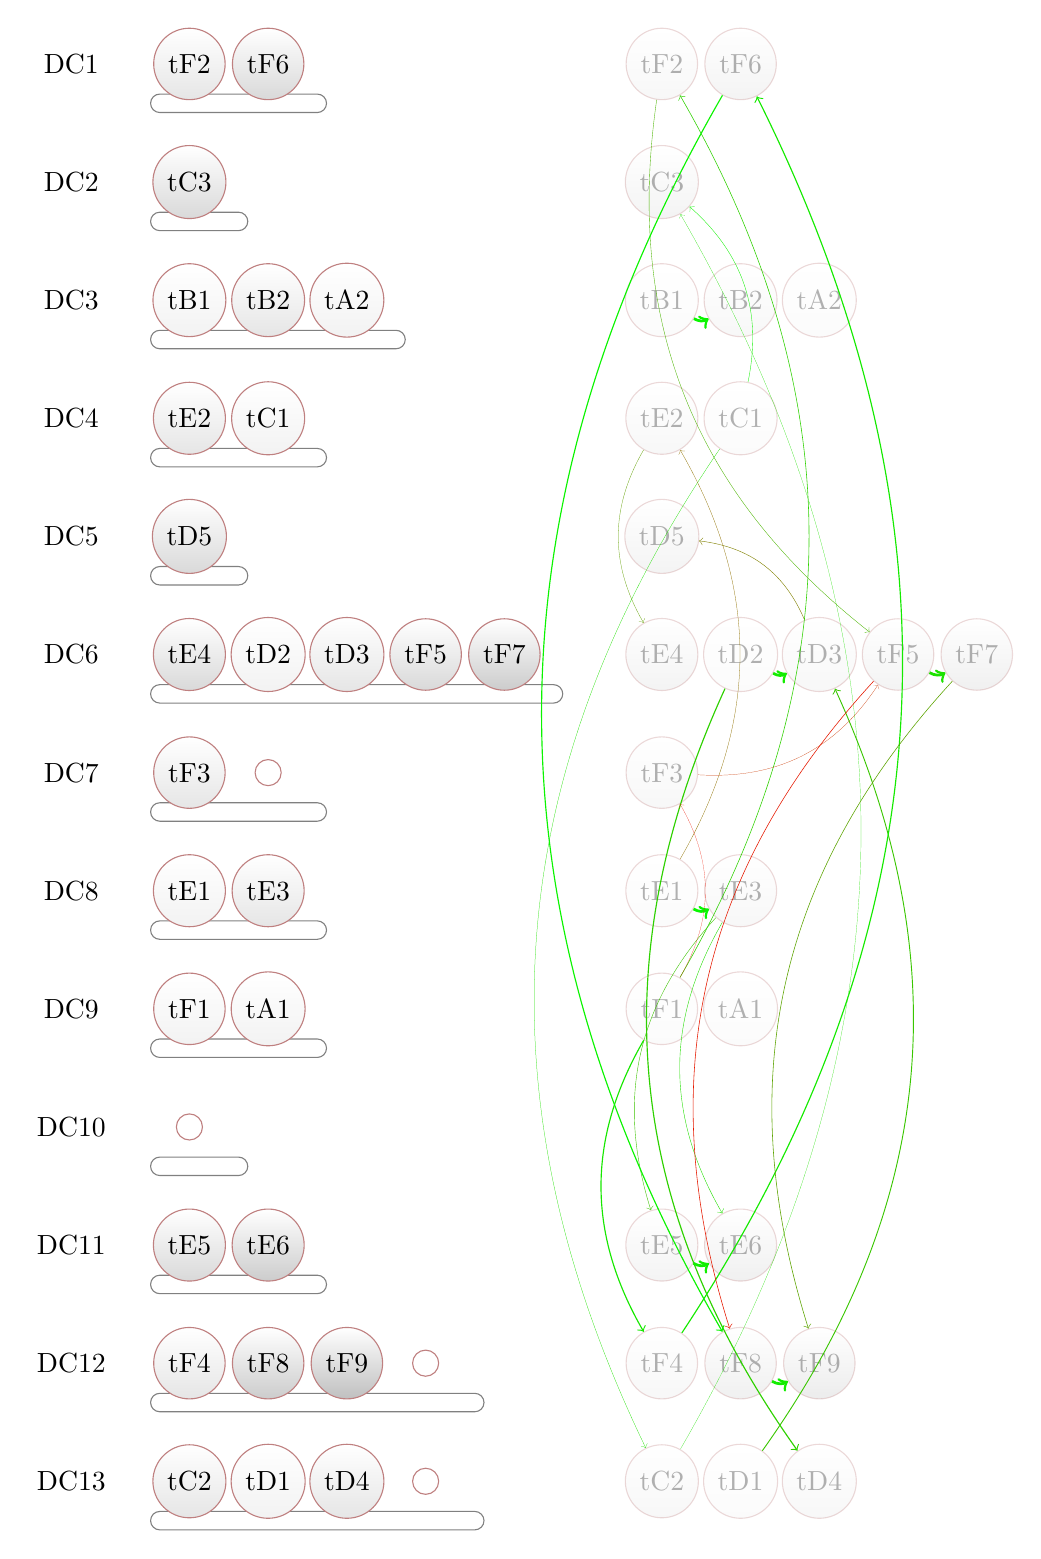
\begin{tikzpicture}
\usetikzlibrary {positioning,shapes.misc}
\tikzstyle{dc} = [rounded rectangle,right,draw=gray,yshift=-0.5cm];
\tikzstyle{task} = [circle,draw=red!50!black!50,top color=white];
\node at (-1.5,0) {DC1};
\node[dc,text width=2.0cm] (DC1) at (-0.5,0) {};
\node[task,bottom color=black!10.0] at (0,0) {tF2};
\node[task,bottom color=black!10.0,opacity=0.3] (tF2) at (6,0) {tF2};
\node[task,bottom color=black!15.0] at (1,0) {tF6};
\node[task,bottom color=black!15.0,opacity=0.3] (tF6) at (7,0) {tF6};
\node at (-1.5,-1.5) {DC2};
\node[dc,text width=1.0cm] (DC2) at (-0.5,-1.5) {};
\node[task,bottom color=black!15.0] at (0,-1.5) {tC3};
\node[task,bottom color=black!15.0,opacity=0.3] (tC3) at (6,-1.5) {tC3};
\node at (-1.5,-3.0) {DC3};
\node[dc,text width=3.0cm] (DC3) at (-0.5,-3.0) {};
\node[task,bottom color=black!5.0] at (0,-3.0) {tB1};
\node[task,bottom color=black!5.0,opacity=0.3] (tB1) at (6,-3.0) {tB1};
\node[task,bottom color=black!10.0] at (1,-3.0) {tB2};
\node[task,bottom color=black!10.0,opacity=0.3] (tB2) at (7,-3.0) {tB2};
\node[task,bottom color=black!5.0] at (2,-3.0) {tA2};
\node[task,bottom color=black!5.0,opacity=0.3] (tA2) at (8,-3.0) {tA2};
\node at (-1.5,-4.5) {DC4};
\node[dc,text width=2.0cm] (DC4) at (-0.5,-4.5) {};
\node[task,bottom color=black!10.0] at (0,-4.5) {tE2};
\node[task,bottom color=black!10.0,opacity=0.3] (tE2) at (6,-4.5) {tE2};
\node[task,bottom color=black!5.0] at (1,-4.5) {tC1};
\node[task,bottom color=black!5.0,opacity=0.3] (tC1) at (7,-4.5) {tC1};
\node at (-1.5,-6.0) {DC5};
\node[dc,text width=1.0cm] (DC5) at (-0.5,-6.0) {};
\node[task,bottom color=black!15.0] at (0,-6.0) {tD5};
\node[task,bottom color=black!15.0,opacity=0.3] (tD5) at (6,-6.0) {tD5};
\node at (-1.5,-7.5) {DC6};
\node[dc,text width=5.0cm] (DC6) at (-0.5,-7.5) {};
\node[task,bottom color=black!15.0] at (0,-7.5) {tE4};
\node[task,bottom color=black!15.0,opacity=0.3] (tE4) at (6,-7.5) {tE4};
\node[task,bottom color=black!5.0] at (1,-7.5) {tD2};
\node[task,bottom color=black!5.0,opacity=0.3] (tD2) at (7,-7.5) {tD2};
\node[task,bottom color=black!10.0] at (2,-7.5) {tD3};
\node[task,bottom color=black!10.0,opacity=0.3] (tD3) at (8,-7.5) {tD3};
\node[task,bottom color=black!15.0] at (3,-7.5) {tF5};
\node[task,bottom color=black!15.0,opacity=0.3] (tF5) at (9,-7.5) {tF5};
\node[task,bottom color=black!20.0] at (4,-7.5) {tF7};
\node[task,bottom color=black!20.0,opacity=0.3] (tF7) at (10,-7.5) {tF7};
\node at (-1.5,-9.0) {DC7};
\node[dc,text width=2.0cm] (DC7) at (-0.5,-9.0) {};
\node[task,bottom color=black!10.0] at (0,-9.0) {tF3};
\node[task,bottom color=black!10.0,opacity=0.3] (tF3) at (6,-9.0) {tF3};
\node[task] at (1,-9.0) {};
\node at (-1.5,-10.5) {DC8};
\node[dc,text width=2.0cm] (DC8) at (-0.5,-10.5) {};
\node[task,bottom color=black!5.0] at (0,-10.5) {tE1};
\node[task,bottom color=black!5.0,opacity=0.3] (tE1) at (6,-10.5) {tE1};
\node[task,bottom color=black!10.0] at (1,-10.5) {tE3};
\node[task,bottom color=black!10.0,opacity=0.3] (tE3) at (7,-10.5) {tE3};
\node at (-1.5,-12.0) {DC9};
\node[dc,text width=2.0cm] (DC9) at (-0.5,-12.0) {};
\node[task,bottom color=black!5.0] at (0,-12.0) {tF1};
\node[task,bottom color=black!5.0,opacity=0.3] (tF1) at (6,-12.0) {tF1};
\node[task,bottom color=black!5.0] at (1,-12.0) {tA1};
\node[task,bottom color=black!5.0,opacity=0.3] (tA1) at (7,-12.0) {tA1};
\node at (-1.5,-13.5) {DC10};
\node[dc,text width=1.0cm] (DC10) at (-0.5,-13.5) {};
\node[task] at (0,-13.5) {};
\node at (-1.5,-15.0) {DC11};
\node[dc,text width=2.0cm] (DC11) at (-0.5,-15.0) {};
\node[task,bottom color=black!15.0] at (0,-15.0) {tE5};
\node[task,bottom color=black!15.0,opacity=0.3] (tE5) at (6,-15.0) {tE5};
\node[task,bottom color=black!20.0] at (1,-15.0) {tE6};
\node[task,bottom color=black!20.0,opacity=0.3] (tE6) at (7,-15.0) {tE6};
\node at (-1.5,-16.5) {DC12};
\node[dc,text width=4.0cm] (DC12) at (-0.5,-16.5) {};
\node[task,bottom color=black!10.0] at (0,-16.5) {tF4};
\node[task,bottom color=black!10.0,opacity=0.3] (tF4) at (6,-16.5) {tF4};
\node[task,bottom color=black!20.0] at (1,-16.5) {tF8};
\node[task,bottom color=black!20.0,opacity=0.3] (tF8) at (7,-16.5) {tF8};
\node[task,bottom color=black!25.0] at (2,-16.5) {tF9};
\node[task,bottom color=black!25.0,opacity=0.3] (tF9) at (8,-16.5) {tF9};
\node[task] at (3,-16.5) {};
\node at (-1.5,-18.0) {DC13};
\node[dc,text width=4.0cm] (DC13) at (-0.5,-18.0) {};
\node[task,bottom color=black!10.0] at (0,-18.0) {tC2};
\node[task,bottom color=black!10.0,opacity=0.3] (tC2) at (6,-18.0) {tC2};
\node[task,bottom color=black!5.0] at (1,-18.0) {tD1};
\node[task,bottom color=black!5.0,opacity=0.3] (tD1) at (7,-18.0) {tD1};
\node[task,bottom color=black!10.0] at (2,-18.0) {tD4};
\node[task,bottom color=black!10.0,opacity=0.3] (tD4) at (8,-18.0) {tD4};
\node[task] at (3,-18.0) {};
\draw[red!3.75!green,line width=1.0pt] (tB1) edge[->,bend right] (tB2);
\draw[red!12.15!green,line width=0.09259259259259259pt] (tC1) edge[->,bend right] (tC2);
\draw[red!6.0!green,line width=0.125pt] (tC1) edge[->,bend right] (tC3);
\draw[red!11.75!green,line width=0.06382978723404255pt] (tC2) edge[->,bend right] (tC3);
\draw[red!22.5!green,line width=0.3333333333333333pt] (tD1) edge[->,bend right] (tD3);
\draw[red!7.5!green,line width=1.0pt] (tD2) edge[->,bend right] (tD3);
\draw[red!18.0!green,line width=0.4166666666666667pt] (tD2) edge[->,bend right] (tD4);
\draw[red!50.0!green,line width=0.15pt] (tD3) edge[->,bend right] (tD5);
\draw[red!56.25!green,line width=0.1pt] (tE1) edge[->,bend right] (tE2);
\draw[red!3.0!green,line width=1.0pt] (tE1) edge[->,bend right] (tE3);
\draw[red!37.5!green,line width=0.1pt] (tE2) edge[->,bend right] (tE4);
\draw[red!23.625!green,line width=0.14285714285714285pt] (tE3) edge[->,bend right] (tE5);
\draw[red!13.125!green,line width=0.14285714285714285pt] (tE3) edge[->,bend right] (tE6);
\draw[red!6.75!green,line width=1.0pt] (tE5) edge[->,bend right] (tE6);
\draw[red!18.0!green,line width=0.20833333333333334pt] (tF1) edge[->,bend right] (tF2);
\draw[red!92.10000000000001!green,line width=0.048859934853420196pt] (tF1) edge[->,bend right] (tF3);
\draw[red!9.0!green,line width=0.4166666666666667pt] (tF1) edge[->,bend right] (tF4);
\draw[red!29.25!green,line width=0.1282051282051282pt] (tF2) edge[->,bend right] (tF5);
\draw[red!78.75000000000001!green,line width=0.07142857142857142pt] (tF3) edge[->,bend right] (tF5);
\draw[red!8.1!green,line width=0.4166666666666667pt] (tF4) edge[->,bend right] (tF6);
\draw[red!11.25!green,line width=1.0pt] (tF5) edge[->,bend right] (tF7);
\draw[red!90.0!green,line width=0.20833333333333334pt] (tF5) edge[->,bend right] (tF8);
\draw[red!4.5!green,line width=0.4166666666666667pt] (tF6) edge[->,bend right] (tF8);
\draw[red!36.0!green,line width=0.20833333333333334pt] (tF7) edge[->,bend right] (tF9);
\draw[red!7.5!green,line width=1.0pt] (tF8) edge[->,bend right] (tF9);
\end{tikzpicture}
\end{document}
